%%%%%%%%%%%%%%%%%%%%%%%%%%%%%%%%%%%%%%%%%%%%%%%%%%%%%%%%%%%%%%%%%%%%%%
% COMP 3804
% February 13, 2012
% Midterm Notes
% By Simon Pratt
%%%%%%%%%%%%%%%%%%%%%%%%%%%%%%%%%%%%%%%%%%%%%%%%%%%%%%%%%%%%%%%%%%%%%%
\documentclass[11pt]{book}

\usepackage{geometry}
\geometry{verbose,tmargin=1in,bmargin=1in,lmargin=.5in,rmargin=.5in}
\usepackage[pdftex]{graphicx}
\usepackage{fancyhdr}
\usepackage{fix-cm}
\usepackage{amsmath}
\usepackage{enumerate}
\usepackage{amsthm}
\usepackage{amssymb}
\usepackage{parskip}
%\usepackage{algorithm}
\usepackage{algorithmic}
\usepackage{multicol}
%\usepackage{newclude} % \include without \clearpage
%\usepackage{ulsy} % needed for \blitza

%%%%%%%%%%%%%%%%%%%%%%%%%%%%%%%%%%%%%%%%%%%%%%%%%%%%%%%%%%%%%%%%%%%%%%
% Question and Answer environments
%%%%%%%%%%%%%%%%%%%%%%%%%%%%%%%%%%%%%%%%%%%%%%%%%%%%%%%%%%%%%%%%%%%%%%

\newcounter{ques}
\newenvironment{question}{\stepcounter{ques}{\bf Question \arabic{ques}:}\vspace{1mm}\fontsize{8}{8}\selectfont}{}
\newenvironment{subquestion}{\fontsize{8}{8}\selectfont}{}
\newenvironment{answer}{{\bf Answer:}\fontsize{12}{12}\selectfont}{}

%%%%%%%%%%%%%%%%%%%%%%%%%%%%%%%%%%%%%%%%%%%%%%%%%%%%%%%%%%%%%%%%%%%%%%
% Theorem, Lemma and Definitions
%%%%%%%%%%%%%%%%%%%%%%%%%%%%%%%%%%%%%%%%%%%%%%%%%%%%%%%%%%%%%%%%%%%%%%

\newtheorem{thm}{Theorem}[ques]
\newtheorem{lem}{Lemma}[ques]
\newtheorem*{bthm}{Theorem}
\theoremstyle{definition}
\newtheorem{dfn}{Definition}
\newtheorem{clm}{Claim}[ques]

%%%%%%%%%%%%%%%%%%%%%%%%%%%%%%%%%%%%%%%%%%%%%%%%%%%%%%%%%%%%%%%%%%%%%%
% Fix for amsthm and parskip
% URL: http://tex.stackexchange.com/questions/22119/how-can-i-change-the-spacing-before-theorems-with-amsthm
%%%%%%%%%%%%%%%%%%%%%%%%%%%%%%%%%%%%%%%%%%%%%%%%%%%%%%%%%%%%%%%%%%%%%%

\makeatletter
\def\thm@space@setup{%
  \thm@preskip=\parskip \thm@postskip=0pt
}
\makeatother

%%%%%%%%%%%%%%%%%%%%%%%%%%%%%%%%%%%%%%%%%%%%%%%%%%%%%%%%%%%%%%%%%%%%%%
% Header/footer
% Mostly taken from: 
%  https://texblog.wordpress.com/2007/11/07/headerfooter-in-latex-with-fancyhdr/
%%%%%%%%%%%%%%%%%%%%%%%%%%%%%%%%%%%%%%%%%%%%%%%%%%%%%%%%%%%%%%%%%%%%%%
\pagestyle{fancyplain}
\setlength{\headheight}{14pt}
\fancyhead{}             % clear header
\fancyfoot{}

\fancyhead[L]{COMP3804}
\fancyhead[C]{Page \thepage }
\fancyhead[R]{Alexis Beingessner \\ Simon Pratt}

%%%%%%%%%%%%%%%%%%%%%%%%%%%%%%%%%%%%%%%%%%%%%%%%%%%%%%%%%%%%%%%%%%%%%%
% Pretty math macros
%%%%%%%%%%%%%%%%%%%%%%%%%%%%%%%%%%%%%%%%%%%%%%%%%%%%%%%%%%%%%%%%%%%%%%
\newcommand{\summ}[2]{\ensuremath{\displaystyle\sum\limits_{#1}^{#2}}} 
%pretty summation

%%%%%%%%%%%%%%%%%%%%%%%%%%%%%%%%%%%%%%%%%%%%%%%%%%%%%%%%%%%%%%%%%%%%%%
% Document
%%%%%%%%%%%%%%%%%%%%%%%%%%%%%%%%%%%%%%%%%%%%%%%%%%%%%%%%%%%%%%%%%%%%%%
\begin{document}
\begin{multicols}{2}
  
  \chapter{Two Fibonaccis}

$fib(n):$
\begin{algorithmic}
\IF { $ n=0 $ or $ n=1 $ }
\RETURN $n$
\ELSE
\RETURN $fib(n-1) + fib(n-2)$
\ENDIF
\end{algorithmic}

We can state a recurrence for this algorithm:

\begin{align*}
T(n) 
&= T(n-1) + T(n-2) + O(1) \\
&\geq fib(n-1) + fib(n-2) \\
&= fib(n)
\end{align*}

$fib2(n):$
\begin{algorithmic}
\IF { $ n = 0 $ }
\RETURN 0
\ENDIF
\STATE create array $f[0 .. n]$
\STATE $f[0] \leftarrow 0, f[1] \leftarrow 1$
\FOR { $ i \leftarrow 2$ to $n$ }
\STATE $f[i] \leftarrow f[i-1] + f[i-2]$
\ENDFOR
\RETURN $f[n]$
\end{algorithmic}

Addition of two numbers in the preceding algorithm takes constant time
until the values exceed the maximum value that can be stored in a
word.  After which, we need to consider how values of arbitrary length
are added.

  \chapter{Integer Multiplication}

Let us consider an integer $X$ which is composed of $X_L$ which are
the leftmost bits of $X$, and $X_R$ which are the rightmost bits of
$X$.

\begin{displaymath}
X = X_L | X_R
\end{displaymath}

We can multiply integers $X,Y$ as follows:

\begin{align*}
XY
&= (2^{n/2}X_L + X_R)(2^{n/2}Y_L + Y_R) \\
&= 2^n X_LY_L + 2^{n/2}X_LY_R + 2^{n/2}X_RY_L + X_RY_R \\
&= 2^n X_LY_L + 2^{n/2}(X_LY_R + X_RY_L) + X_RY_R \\
\end{align*}

Which gives the recurrence

\begin{align*}
T(n)
&= 4T(n/2) + O(n) \\
&\leq 4T(n/2) + cn \\
&\leq 4(4T(n/4) + cn/2) + cn \\
&\leq 4(4(4T(n/8) + cn/4) + cn/2) + cn \\
&\leq 64T(n/8) + cn(1 + 2 + 4) \\
&... \\
&\leq 4^iT(n/2^i) + cn(1 + 2 + ... + 2^{i-1})
\end{align*}

Where $i$ is the number of times we can divide $n$ by 2, or $log_2n$.

\begin{align*}
T(n)
&\leq 4^{log_2n}T(n/2^{log_2n}) + cn(1 + 2 + ... + 2^{log_2n-1}) \\
&\leq n^{log_24}T(n/n^{log_22}) + cn \summ{i=0}{log_2n-1} 2^i \\
&\leq n^2T(1) + cn 2^{log_2n} \\
&\leq n^2T(1) + cn n^{log_22} \\
&\leq n^2T(1) + cn^2 \\
&\leq n^2(T(1) + c) \\
&\leq n^2(O(1) + c) \\
&\leq O(n^2)
\end{align*}

Can we do better?  Yes.

We need: $X_LY_L, X_RY_R,$ and $X_LY_R + X_RY_L$

Observe: 
%
\begin{align*}
&(X_L + X_R)(Y_L + Y_R) - X_LY_L - X_RY_R \\
&= X_LY_L + X_RY_L + X_LY_R + X_RY_R - X_LY_L - X_RY_R \\
&= X_RY_L + X_LY_R
\end{align*}

Since we must compute $X_LY_L$ and $X_RY_R$ anyway, this saves us an
entire multiplication.  Reducing our recurrence from $T(n) = 4T(n/2) +
O(n)$ to $T(n) = 3T(n/2) + O(n)$.

We can solve this new recurrence as follows:

\begin{align*}
T(n)
&= 3T(n/2) + O(n) \\
&\leq 3T(n/2) + cn \\
&\leq 3(3T(n/4) + cn/2) + cn \\
&\leq 3^iT(n/2^i) + cn(1 + 3/2 + ... + (3/2)^{i-1}) \\
&\leq 3^{log_2n}T(n/2^{log_2n}) + cn(1 + 2 + ... + (3/2)^{log_2n-1}) \\
&\leq n^{log_23}T(1) + cn \summ{i=0}{log_2n-1} (3/2)^i \\
&\leq n^{log_23}T(1) + cn (3/2)^{log_2n} \\
&\leq n^{log_23}T(1) + cn n^{log_2(3/2)} \\
&\leq n^{log_23}T(1) + cn n^{log_23 - log_22} \\
&\leq n^{log_23}T(1) + cn n^{log_23 - 1} \\
&\leq n^{log_23}T(1) + cn n^{log_23}n^{-1} \\
&\leq n^{log_23}(T(1) + cn/n) \\
&\leq n^{log_23}(T(1) + c) \\
&\leq O(n^{log_23})
\end{align*}

  \chapter{Solving Recurrences}

\section{The Master Theorem}

If $T(n) = aT(\frac{n}{b}) + O(n^d)$, then

\begin{math}
T(n) = \left\{
\begin{array}{l l}
O(n^d)       & \quad \text{if} d > log_ba \\
O(n^d logn)  & \quad \text{if} d = log_ba \\
O(n^{log_ba}) & \quad \text{if} d < log_ba \\
\end{array} \right.
\end{math}

\section{Recursion Tree}

We can reason about a recurrence of the form: $ T(n) = aT(\frac{n}{b})
+ f(n) $ where $ a \geq 0, b > 0 $ with the following recursion tree:

{
  % Current graphic is hand-drawn by John Howat.
  % Should replace asap with a nicer diagram
  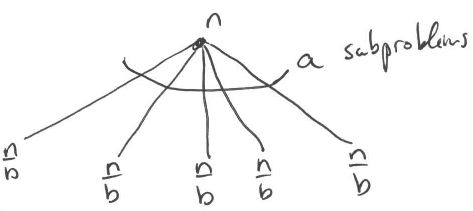
\includegraphics[scale=1.2]{recursion_tree}
  %\caption{A recursion tree representing a recursions on n/b elements}
  \label{fig:recursion_tree}
}

This tree has the following properties:

\begin{enumerate}
\item The number of nodes at level $i$: $a^i$
\item Work done at each node of level $i$: $f(\frac{n}{b^i})$
\item Number of levels: $log_bn$
\item Number of leaves: $n^{log_ba}$
\end{enumerate}

We can use this information to solve the recurrence:

\begin{align*}
T(n)
&= \sum\limits_{i=0}^{log_bn} 
(\text{\# nodes at level } i) 
(\text{work done at level } i) \\
&= \sum\limits_{i=0}^{log_bn} a^i f(\frac{n}{b^i})
\end{align*}

  \chapter{Heaps}

For the purposes of generality, instead of referring to 
elements that are ``greater than" or ``less than" others,
we will simply say that they are ``better than" or ``worse than"
others. For any particular ordering, the ``best" element is desired first.
A Heap is a binary tree that satisfies the following properties:

\begin{itemize}
\item The root of a heap is better than its two children (the heap property)
\item The children of the root are also heaps  
\item A heap is a complete binary tree (only the last level may not be full, 
and all elements in the last level are on the left)
\end{itemize}

A heap differs from most binary trees in that it provides no particular
ordering of the elements, but rather guarantees that the best element is
at the root. Further, while heaps are usually discussed and defined
as binary trees, they need not be implemented as such.
A heap can in fact be implemented as an array with no performance reduction.
To do so, we can implement a simple indexing. If an element is at the $i$th
index in the array, it's left and right child are at the $2i+1$th and $2i+2$th 
indexes respectively. By placing the root at the $0$th index, all others follow.
This is depicted below.
{
  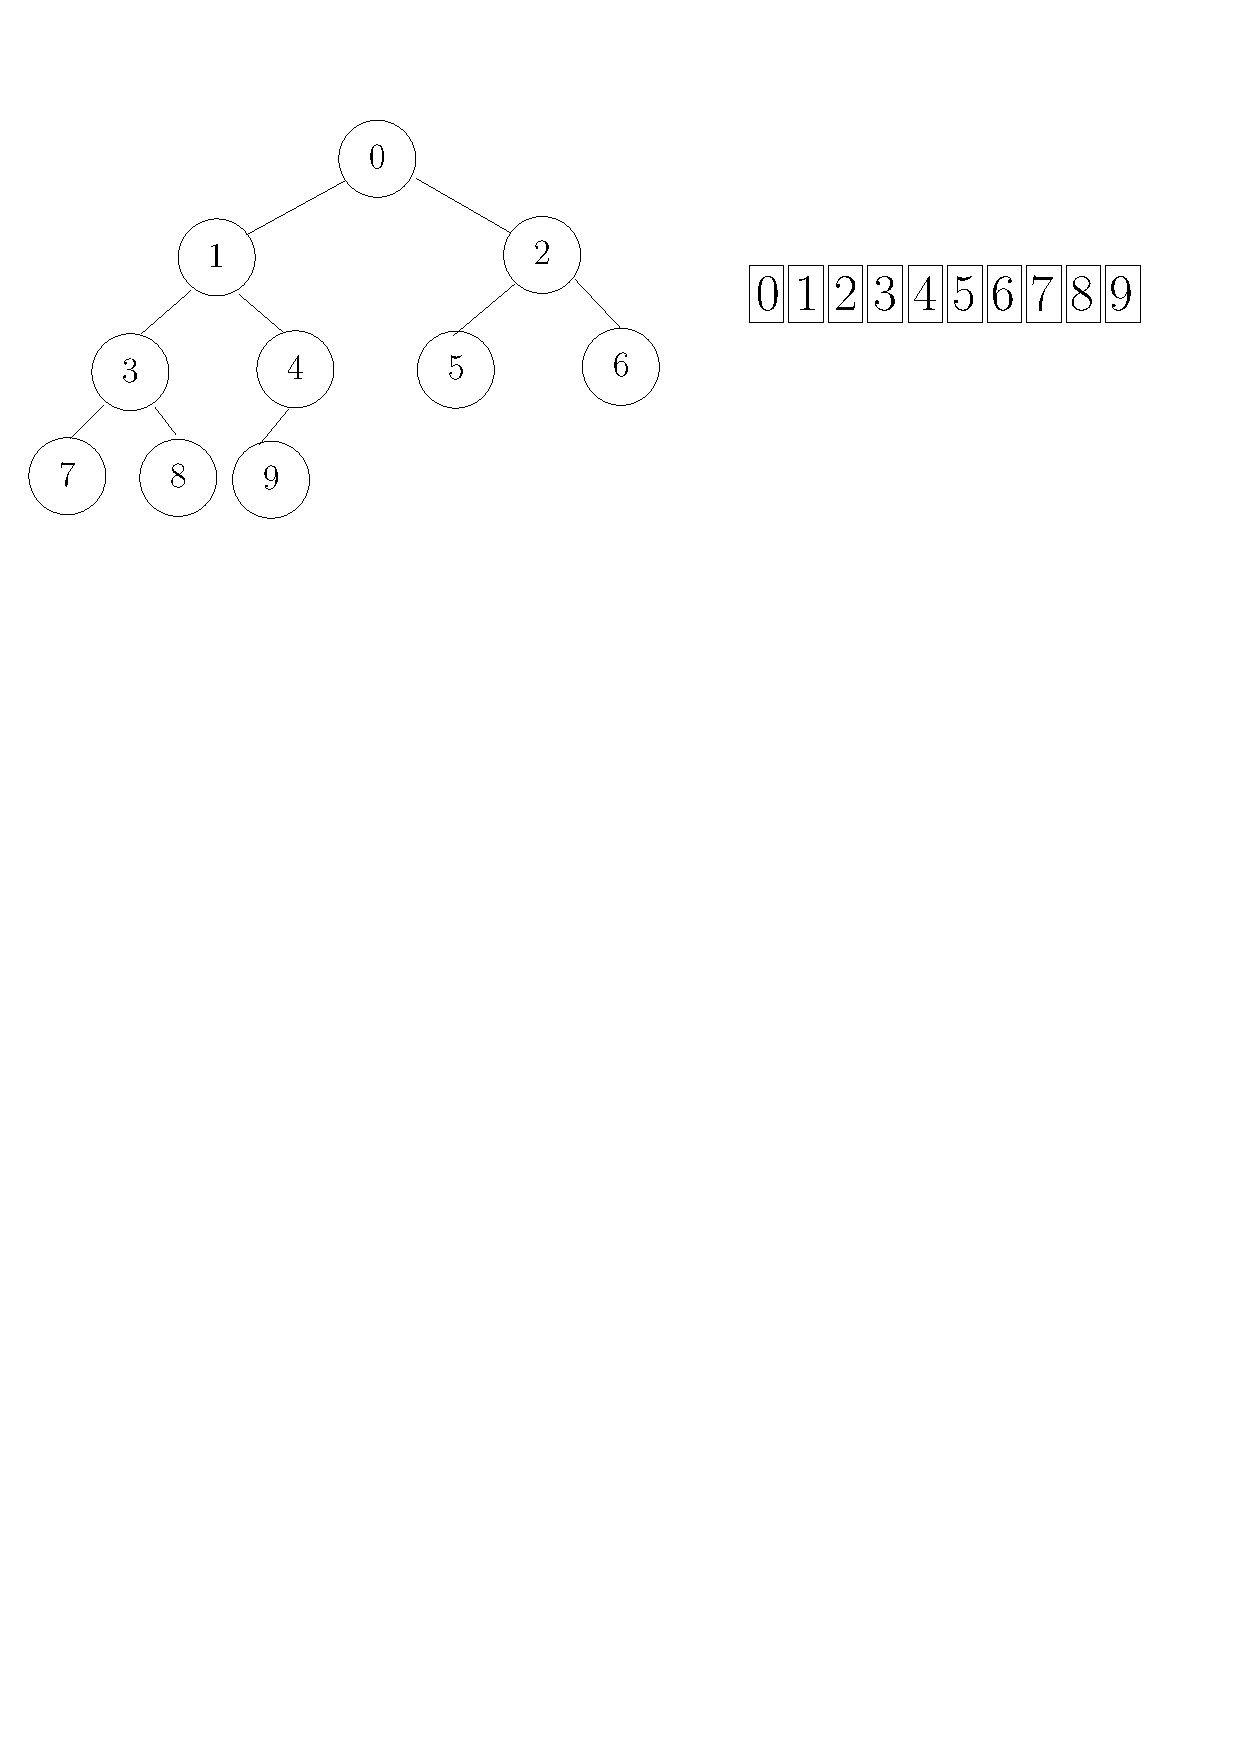
\includegraphics[scale=0.5]{heapTreeArray}
  %\caption{The mapping of a binary tree to an array}
  \label{fig:heapTreeArray}
}
Heaps are commonly used to implement priority queues, because they do the
minimum amount of work required to keep track of the best element.

\section{How to Implement a Heap}

A heap must support the following operations

\begin{itemize}
\item $best()$: returns the best element in the heap
\item $pop-best()$: removes the best element in the heap
\item $insert(x)$: inserts $x$ into the heap
\end{itemize}

From the definition of a heap, we know the we can easily implement
$best()$ by returning the root of the heap, which should take $O(1)$ time.
However the other operations are less obvious. 

To $insert(x)$ recall that a heap must be complete, therefore, if a new
element is added, it must be added to the left-most available space in the
last row of the heap. However, the heap property may now be violated. 
If the new element $x$ is worse than its parent $y$, the heap property is
satisfied and we may stop. However if it is not satisfied we may swap
$x$ with $y$ and recurse on $x$'s new position. This works because we know
that $y$ is better than all of $x$'s children, because the heap property was
satisfied before $x$ was added. Further, because $x$ is better than $y$, it
is also better than all of $y$'s children. However $x$ may still be better than
its new parent, so we must recurse. If $x$ is the new best element, it will
eventually reach the root. Because heaps are complete, this operation will take
$O(\log n)$ time, as this is the height of the heap.

To $pop-best()$, we may simply remove the root,
however this completely destroys the entire heap. Instead, we will swap
the root with the bottom-left-most element, $y$. Now removing the
best element leaves us with a still complete tree. However the heap property
has likely been violated once more. If $y$ is better than both its children,
then we may stop. However, if not, we shall swap $y$ with its largest child
and recurse on $y's$ new position. Because the element we swap with $y$ is
better than both $y$ and the other child, the heap property has been
satisfied for this sub-heap. However, the heap property may still be violated
for $y's$ new sub-heap, so we must do this again, until $y$ is the root
of a valid heap. Once more, this operation
requires $O(\log n)$ time, as it must at worse traverse the entire height
of the tree. 

Therefore, a heap may support $best()$ in $O(1)$ time, $insert(x)$ 
in $O(\log n)$ time, and $pop-best()$ in $O(\log n)$ time.

\section{Building a Heap}

Now that we can support all the operations that a heap must implement,
it would be nice to be able to actually construct one given a list of $n$
elements. A naive approach is to simply call $insert(x)$ on every element
in the list. However, since $insert(x)$ requires $O(\log n)$ time, this will
require $O(n \log n)$ time. These seems pretty bad, considering one can find
the best element in a list by brute force in $O(n)$ time. Can we achieve a
construction time comparable to the brute force time?
Instead of building the heap top down with $insert$, we can build it from the
bottom up. Remark that a single element is a valid heap. If we were to try to
build from the bottom up, we could first take the last $n/2$ elements in the
list. All of these elements are their own valid and complete heaps,
and we therefore do not need to do anything to them.
To add the next $n/4$ elements, we simply perform
the procedure we did in $pop-best$ to fix the fact that the new root might
be violating the heap property, knowing that all the elements below it are
valid heaps. By repeating this process until we reach the first element in
the list, we will have created a valid heap on $n$ elements.

Because we are doing very little work for the majority of the elements, we end
up doing only $O(n)$ work over all, which is optimal, as this is the amount of
time required to find the best element.

\section{Heapsort}

Another nice property of a heap is that once one has been implemented,
it provides a very simple procedure for sort elements.
A simple algorithm to do this to construct a heap on the list and then simply
return $best$ and then call $pop-best$ over and over until there are no more
elements in the heap.
In fact, since our algorithm for building the heap is in-place and takes $O(n)$
time, and our remove method leaves the best element at the end of the array,
by simply building a heap on the input array and calling $pop-best$ $n$ times,
we will be left with a reverse sorted array in $O(n \log n)$ time. 
This algorithm is particularly excellent because it requires no extra space,
runs deterministically, and is worst-case optimal.



\end{multicols}
\end{document}
